\chapter{Mathematical Review}

Set theory is generally accepted as the foundation of modern mathematics, and it plays an instrumental role in the treatment of probability.
Unfortunately, a simple description of set theory can lead to paradoxes, while a rigorous axiomatic approach is quite tedious.
In these notes, we circumvent these difficulties and assume that the meaning of a set as a collection of objects is intuitively clear.
This standpoint is known as naive set theory.
From here, we proceed to define relevant notation and operations.

\begin{figure}[htb]
\begin{center}
% FIGURE GROUP = BALLS
\begin{footnotesize}
\begin{tikzpicture}
\draw[color=black, thick, dashed] (0,0) ellipse (30mm and 20mm);

\shade[draw=black, ball color=red, circular drop shadow] (0.75,1.25) circle (4mm);
\shade[fill=white, fill opacity=0.3] (0.75,1.25) circle (4mm) node[fill opacity=1]{1};

\shade[draw=black, ball color=blue, circular drop shadow] (-2,0.25) circle (4mm);
\shade[fill=white, fill opacity=0.3] (-2,0.25) circle (4mm) node[fill opacity=1]{2};

\shade[draw=black, ball color=green, circular drop shadow] (-1,1) circle (4mm);
\shade[fill=white, fill opacity=0.3] (-1,1) circle (4mm) node[fill opacity=1]{3};

\shade[draw=black, ball color=gray, circular drop shadow] (2.25,0) circle (4mm);
\shade[fill=white, fill opacity=0.3] (2.25,0) circle (4mm) node[fill opacity=1]{4};

\shade[draw=black, ball color=cyan, circular drop shadow] (0,-0.25) circle (4mm);
\shade[fill=white, fill opacity=0.3] (0,-0.25) circle (4mm) node[fill opacity=1]{5};

\shade[draw=black, ball color=magenta, circular drop shadow] (1.25,-0.75) circle (4mm);
\shade[fill=white, fill opacity=0.3] (1.25,-0.75) circle (4mm) node[fill opacity=1]{6};

\shade[draw=black, ball color=yellow, circular drop shadow] (-1.25,-1) circle (4mm);
\shade[fill=white, fill opacity=0.3] (-1.25,-1) circle (4mm) node[fill opacity=1]{7};
\end{tikzpicture}
\end{footnotesize}
\caption{This is an illustration of a generic set and its elements.}
\end{center}
\end{figure}

A \emph{set} is a collection of objects, which are called the \emph{elements} of the set.\index{Set}\index{Element}
If an element $x$ belongs to a set $S$, we express this fact by writing $x \in S$.
If $x$ does not belong to $S$, we write $x \notin S$.
We use the equality symbol to denote \emph{logical identity}.
For instance, $x = y$ means that $x$ and $y$ are symbols denoting the same object.
Similarly, the equation $S = T$ states that $S$ and $T$ are two symbols for the same set.
In particular, the sets $S$ and $T$ contain precisely the same elements.
If $x$ and $y$ are different objects then we write $x \neq y$.
Also, we can express the fact that $S$ and $T$ are different sets by writing $S \neq T$.

A set $S$ is a \emph{subset} of $T$ if every element of $S$ is also contained in $T$.\index{Subset}
We express this relation by writing $S \subset T$.
Note that this definition does not require $S$ to be different from $T$.
If $S \subset T$ and $S$ is different from $T$, then $S$ is a \emph{proper subset} of $T$, which we indicate by $S \subsetneq T$.\index{Proper subset}
Moreover, $S = T$ if and only if $S \subset T$ and $T \subset S$.
In fact, this latter statement outlines a methodology to show that two sets are equal.

There are many ways to specify a set.
If the set contains only a few elements, one can simply list the objects in the set;
\begin{equation*}
S = \{ x_1, x_2, x_3 \} .
\end{equation*}
The content of a set can also be enumerated whenever $S$ has a countable number of elements,
\begin{equation*}
S = \{ x_1, x_2, \ldots \} .
\end{equation*}
Usually, the way to specify a set is to take some collection $T$ of objects and some property that elements of $T$ may or may not possess, and to form the set consisting of all elements of $T$ having that property.
For example, starting with the integers $\Integers$, we can form the subset $S$ consisting of all even numbers,
\begin{equation*}
S = \{ x \in \Integers | x \text{ is an even number} \}.
\end{equation*}
More generally, we denote the set of all elements that satisfy a certain property $P$ by $S = \{ x | x \text{ satisfies } P \}$.
The braces are to be read as ``the set of'' while the symbol $|$ stands for the words ``such that.''

It is convenient to introduce two special sets.
The \emph{empty set}, denoted by $\emptyset$, is a set that contains no elements.\index{Empty set}
The \emph{universal set} is the collection of all objects of interest in a particular context, and it is represented by $\Omega$.
Once a universal set $\Omega$ is specified, we need only consider sets that are subsets of $\Omega$.
In the context of probability, $\Omega$ is often called the \emph{sample space}.\index{Sample space}
The \emph{complement} of a set $S$, relative to the universal set $\Omega$, is the collection of all objects in $\Omega$ that do not belong to $S$,\index{Complement}
\begin{equation*}
S^{\Complement} = \{ x \in \Omega | x \notin S \}.
\end{equation*}
For example, we have $\Omega^{\Complement} = \emptyset$.


\section{Elementary Set Operations}

The field of probability makes extensive use of set theory.
Below, we review elementary set operations, and we establish basic terminology and notation.
Consider two sets, $S$ and $T$.

\begin{figure}[htb!]
\begin{center}
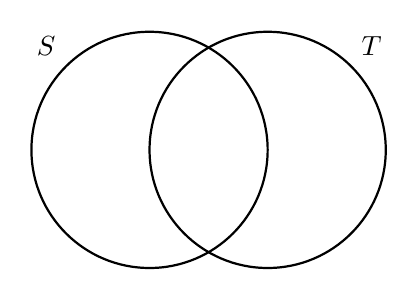
\begin{tikzpicture}
\node[circle,draw=black,thick,minimum size=3cm,label=135:$S$] (S) at (-0.75cm,0) {};
\node[circle,draw=black,thick,minimum size=3cm,label=45:$T$] (T) at (0.75cm,0) {};
\end{tikzpicture}
\caption{This is an abstract representation of two sets, $S$ and $T$.
Each set contains the elements located in its shaded circle and the overlap corresponds to elements that are in both sets.}
\end{center}
\end{figure}

The \emph{union} of sets $S$ and $T$ is the collection of all elements that belong to $S$ or $T$ (or both), and it is denoted by $S \cup T$.\index{Union}
Formally, we define the union of these two sets by $S \cup T = \{ x | x \in S \text{ or } x \in T \}$.

\begin{figure}[htb!]
\begin{center}
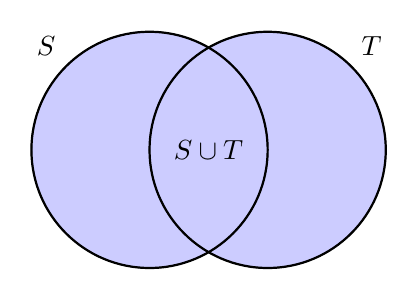
\begin{tikzpicture}
\draw[fill=blue!20]
	(-0.75cm,0) circle (1.5cm)
	(0.75cm,0) circle (1.5cm);
\node[circle,draw=black,thick,minimum size=3cm,label=135:$S$] (S) at (-0.75cm,0) {};
\node[circle,draw=black,thick,minimum size=3cm,label=45:$T$] (T) at (0.75cm,0) {};
\coordinate [label=center:{$S \cup T$}] (Union) at (0,0);
\end{tikzpicture}
\caption{The union of sets $S$ and $T$ consists of all elements that are contained in $S$ or $T$.}
\end{center}
\end{figure}

The \emph{intersection} of sets $S$ and $T$ is the collection of all elements that belong to both $S$ and $T$.\index{Intersection}
It is denoted by $S \cap T$, and it can be expressed mathematically as $S \cap T = \{ x | x \in S \text{ and } x \in T \}$.

\begin{figure}[htb!]
\begin{center}
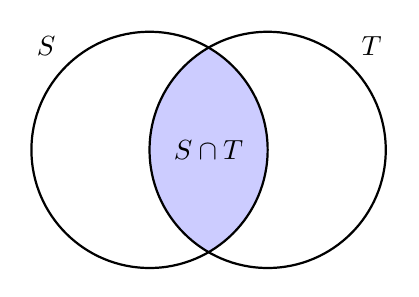
\begin{tikzpicture}
\begin{scope}
	\clip (-0.75cm,0) circle (1.5cm);
	\fill[fill=blue!20] (0.75cm,0) circle (1.5cm);
\end{scope}
\node[circle,draw=black,thick,minimum size=3cm,label=135:$S$] (S) at (-0.75cm,0) {};
\node[circle,draw=black,thick,minimum size=3cm,label=45:$T$] (T) at (0.75cm,0) {};
\coordinate [label=center:{$S \cap T$}] (Intersection) at (0,0);
\end{tikzpicture}
\caption{The intersection of sets $S$ and $T$ only contains elements that are both in $S$ and $T$.}
\end{center}
\end{figure}

When $S$ and $T$ have no elements in common, we write $S \cap T = \emptyset$.
We also express this fact by saying that $S$ and $T$ are \emph{disjoint}.\index{Disjoint sets}
More generally, a collection of sets is said to be disjoint if no two sets have a common element.
A collection of sets is said to form a \emph{partition} of $S$ if the sets in the collection are disjoint and their union is $S$.\index{Partition}

\begin{figure}[htb]
\begin{center}
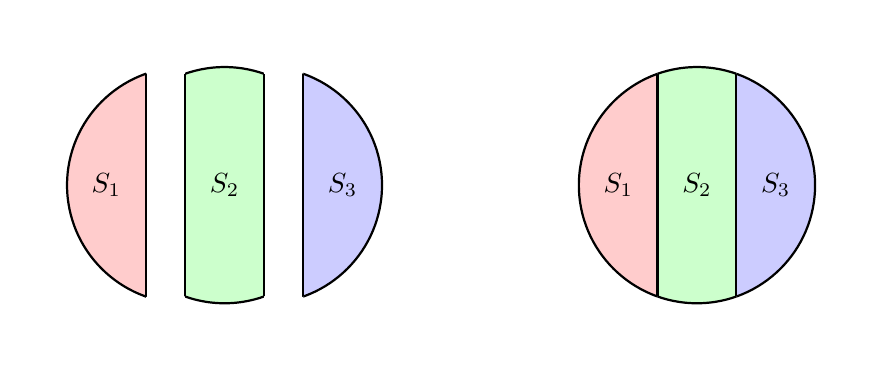
\begin{tikzpicture}
\begin{scope}
	\clip (-0.5cm,-2cm) rectangle (0.5cm,2cm);
	\draw[thick,fill=green!20] (0,0) circle (1.5cm);
\end{scope}
\begin{scope}
	\clip (0,0) circle (1.5cm);
	\draw[thick] (-0.5cm,-2cm) rectangle (0.5cm,2cm);
\end{scope}
\begin{scope}
	\clip (-2.5cm,-2cm) rectangle (-1cm,2cm);
	\draw[thick,fill=red!20] (-0.5cm,0) circle (1.5cm);
\end{scope}
\begin{scope}
	\clip (-0.5cm,0) circle (1.5cm);
	\draw[thick] (-2.5cm,-2cm) rectangle (-1cm,2cm);
\end{scope}
\begin{scope}
	\clip (1cm,-2cm) rectangle (2.5cm,2cm);
	\draw[thick,fill=blue!20] (0.5cm,0) circle (1.5cm);
\end{scope}
\begin{scope}
	\clip (0.5cm,0) circle (1.5cm);
	\draw[thick] (1cm,-2cm) rectangle (2.5cm,2cm);
\end{scope}
\coordinate [label=center:{$S_1$}] (S1a) at (-1.5cm,0);
\coordinate [label=center:{$S_2$}] (S2a) at (0,0);
\coordinate [label=center:{$S_3$}] (S3a) at (1.5cm,0);

\begin{scope}
	\clip (5.5cm,-2cm) rectangle (6.5cm,2cm);
	\draw[thick,fill=green!20] (6cm,0) circle (1.5cm);
\end{scope}
\begin{scope}
	\clip (4cm,-2cm) rectangle (5.5cm,2cm);
	\draw[thick,fill=red!20] (6cm,0) circle (1.5cm);
\end{scope}
\begin{scope}
	\clip (6.5cm,-2cm) rectangle (8cm,2cm);
	\draw[thick,fill=blue!20] (6cm,0) circle (1.5cm);
\end{scope}
\begin{scope}
	\clip (6cm,0) circle (1.5cm);
	\draw[thick] (5.5cm,-2cm) rectangle (6.5cm,2cm);
\end{scope}
\coordinate [label=center:{$S_1$}] (S1b) at (5cm,0);
\coordinate [label=center:{$S_2$}] (S2b) at (6cm,0);
\coordinate [label=center:{$S_3$}] (S3b) at (7cm,0);
\end{tikzpicture}
\caption{A partition of $S$ is a collection of sets that are disjoint and whose union is $S$.
Above, $S$ is partition into three disjoint subsets: $S_1$, $S_2$, and $S_3$.}
\end{center}
\end{figure}

The \emph{difference} of two sets, denoted by $S - T$, is defined as the set consisting of those elements of $S$ that are not in $T$, $S - T = \{ x | x \in S \text{ and } x \notin T \}$.
This set is sometimes called the complement of $T$ relative to $S$, or the complement of $T$ in $S$.

\begin{figure}[htb]
\begin{center}
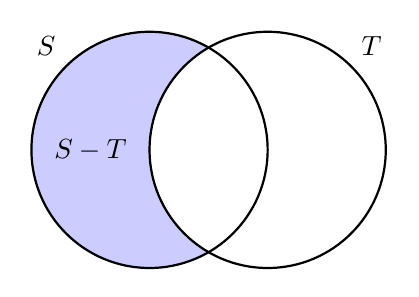
\begin{tikzpicture}
\begin{scope}
	\clip (-0.75cm,0) circle (1.5cm);
	\draw[fill=blue!20,even odd rule]
	(0.75cm,0) circle (1.5cm)
	(-0.75cm,0) circle (1.5cm);
\end{scope}
\node[circle,draw=black,thick,minimum size=3cm,label=135:$S$] (S) at (-0.75cm,0) {};
\node[circle,draw=black,thick,minimum size=3cm,label=45:$T$] (T) at (0.75cm,0) {};
\coordinate [label=center:{$S - T$}] (Difference) at (-1.5cm,0);
\end{tikzpicture}
\caption{The complement of $T$ relative to $S$ contains all the elements of $S$ that are not in $T$.}
\end{center}
\end{figure}

So far, we have looked at the definition of the union and the intersection of two sets.
We can also form the union or the intersection of arbitrarily many sets.
This is defined in a straightforward way,
\begin{align*}
\bigcup_{i \in \IndexSet} S_{i}
&= \{ x | x \in S_{i} \text{ for some } i \in \IndexSet \} \\
\bigcap_{i \in \IndexSet} S_{i}
&= \{ x | x \in S_{i} \text{ for all } i \in \IndexSet \} .
\end{align*}
The index set $\IndexSet$ can be finite or infinite.


\section{Additional Rules and Properties}

Given a collection of sets, it is possible to form new ones by applying elementary set operations to them.
As in algebra, one uses parentheses to indicate precedence.
For instance, $R \cup (S \cap T)$ denotes the union of two sets $R$ and $S \cap T$, whereas $(R \cup S) \cap T$ represents the intersection of two sets $R \cup S$ and $T$.
The sets thus formed are quite different.

\begin{figure}[htb]
\begin{center}
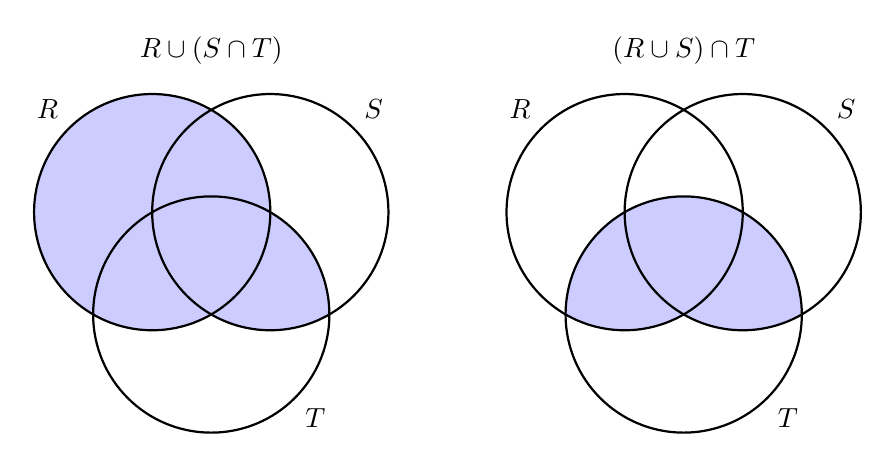
\begin{tikzpicture}
\begin{scope}
	\clip (0.75cm,0) circle (1.5cm);
	\fill[fill=blue!20] (0,-1.3cm) circle (1.5cm);
\end{scope}
\fill[blue!20] (-0.75cm,0) circle (1.5cm);
\node[circle,draw=black,thick,minimum size=3cm,label=135:$R$] (R1) at (-0.75cm,0) {};
\node[circle,draw=black,thick,minimum size=3cm,label=45:$S$] (S1) at (0.75cm,0) {};
\node[circle,draw=black,thick,minimum size=3cm,label=315:$T$] (T1) at (0,-1.3cm) {};
\coordinate [label={$R \cup (S \cap T)$}] (Cap1) at (0,1.75cm);

\begin{scope}
	\clip (6.75cm,0) circle (1.5cm);
	\fill[fill=blue!20] (6,-1.3cm) circle (1.5cm);
\end{scope}
\begin{scope}
	\clip (5.25cm,0) circle (1.5cm);
	\fill[fill=blue!20] (6,-1.3cm) circle (1.5cm);
\end{scope}
\node[circle,draw=black,thick,minimum size=3cm,label=135:$R$] (R2) at (5.25cm,0) {};
\node[circle,draw=black,thick,minimum size=3cm,label=45:$S$] (S2) at (6.75cm,0) {};
\node[circle,draw=black,thick,minimum size=3cm,label=315:$T$] (T2) at (6cm,-1.3cm) {};
\coordinate [label={$(R \cup S) \cap T$}] (Cup1) at (6,1.75cm);
\end{tikzpicture}
\caption{The order of set operations is important; parentheses should be employed to specify precedence.}
\end{center}
\end{figure}

Sometimes, different combinations of operations lead to a same set.
For instance, we have the following distributive laws
\begin{align*}
R \cap (S \cup T) &= (R \cap S) \cup (R \cap T) \\
R \cup (S \cap T) &= (R \cup S) \cap (R \cup T).
\end{align*}
Two particularly useful equivalent combinations of operations are given by \emph{De~Morgan's laws}, which state that\index{De Morgan's laws}
\begin{align*}
R - (S \cup T) &= (R - S) \cap (R - T) \\
R - (S \cap T) &= (R - S) \cup (R - T).
\end{align*}
These two laws can also appear in different forms,
\begin{align*}
\left( \bigcup_{i \in \IndexSet} S_{i} \right)^{\Complement}
&= \bigcap_{i \in \IndexSet} S_{i}^{\Complement} \\
\left( \bigcap_{i \in \IndexSet} S_{i} \right)^{\Complement}
&= \bigcup_{i \in \IndexSet} S_{i}^{\Complement}
\end{align*}
when multiple sets are involved.
To establish the first equality, suppose that $x$ belongs to $\left( \bigcup_{i \in \IndexSet} S_{i} \right)^{\Complement}$.
Then $x$ is not contained in $\bigcup_{i \in \IndexSet} S_{i}$.
That is, $x$ is not an element of $S_{i}$ for any $i \in \IndexSet$.
This implies that $x$ belongs to $S_{i}^{\Complement}$ for all $i \in \IndexSet$, and therefore $x \in \bigcap_{i \in \IndexSet} S_{i}^{\Complement}$.
We have shown that $\left( \bigcup_{i \in \IndexSet} S_{i} \right)^{\Complement} \subset \bigcap_{i \in \IndexSet} S_{i}^{\Complement}$.
The converse inclusion is obtained by reversing the above argument.
The second law can be obtained in a similar fashion.


\section{Cartesian Products}

There is yet another way to create new sets from existing ones.
It involves the notion of an \emph{ordered pair} of objects.\index{Ordered pair}
Given sets $S$ and $T$, the \emph{cartesian product} $S \times T$ is the set of all ordered pairs $(x, y)$ such that $x$ is an element of $S$ and $y$ is an element of $T$, $S \times T = \{ (x, y) | x \in S \text{ and } y \in T \}$.\index{Cartesian product}

\begin{figure}[htb]
\begin{center}
% FIGURE GROUP = BALLS
\begin{footnotesize}
\begin{tikzpicture}
\shade[draw=black, ball color=red, circular drop shadow] (0,1.25) circle (4mm);
\shade[fill=white, fill opacity=0.3] (0,1.25) circle (4mm) node[fill opacity=1]{1};

\shade[draw=black, ball color=blue, circular drop shadow] (0,0) circle (4mm);
\shade[fill=white, fill opacity=0.3] (0,0) circle (4mm) node[fill opacity=1]{2};

\shade[draw=black, ball color=green, circular drop shadow] (0,-1.25) circle (4mm);
\shade[fill=white, fill opacity=0.3] (0,-1.25) circle (4mm) node[fill opacity=1]{3};

\draw[very thick] (0.85,-0.2) -- (1.25,0.2);
\draw[very thick] (0.85,0.2) -- (1.25,-0.2);

\shade[draw=black, ball color=yellow, circular drop shadow] (2,0.75) circle (4mm);
\shade[fill=white, fill opacity=0.3] (2,0.75) circle (4mm) node[fill opacity=1]{$\mathrm{a}$};

\shade[draw=black, ball color=magenta, circular drop shadow] (2,-0.75) circle (4mm);
\shade[fill=white, fill opacity=0.3] (2,-0.75) circle (4mm) node[fill opacity=1]{$\mathrm{b}$};

\draw[very thick, ->, >=stealth'] (3,0) -- (4,0);

\shade[draw=black, ball color=red, circular drop shadow] (5,1.25) circle (4mm);
\shade[fill=white, fill opacity=0.3] (5,1.25) circle (4mm) node[fill opacity=1]{1};
\shade[draw=black, ball color=yellow, circular drop shadow] (5.9,1.25) circle (4mm);
\shade[fill=white, fill opacity=0.3] (5.9,1.25) circle (4mm) node[fill opacity=1]{$\mathrm{a}$};

\shade[draw=black, ball color=red, circular drop shadow] (5,0) circle (4mm);
\shade[fill=white, fill opacity=0.3] (5,0) circle (4mm) node[fill opacity=1]{1};
\shade[draw=black, ball color=magenta, circular drop shadow] (5.9,0) circle (4mm);
\shade[fill=white, fill opacity=0.3] (5.9,0) circle (4mm) node[fill opacity=1]{$\mathrm{b}$};

\shade[draw=black, ball color=blue, circular drop shadow] (5,-1.25) circle (4mm);
\shade[fill=white, fill opacity=0.3] (5,-1.25) circle (4mm) node[fill opacity=1]{2};
\shade[draw=black, ball color=yellow, circular drop shadow] (5.9,-1.25) circle (4mm);
\shade[fill=white, fill opacity=0.3] (5.9,-1.25) circle (4mm) node[fill opacity=1]{$\mathrm{a}$};

\shade[draw=black, ball color=blue, circular drop shadow] (7.5,1.25) circle (4mm);
\shade[fill=white, fill opacity=0.3] (7.5,1.25) circle (4mm) node[fill opacity=1]{2};
\shade[draw=black, ball color=magenta, circular drop shadow] (8.4,1.25) circle (4mm);
\shade[fill=white, fill opacity=0.3] (8.4,1.25) circle (4mm) node[fill opacity=1]{$\mathrm{b}$};

\shade[draw=black, ball color=green, circular drop shadow] (7.5,0) circle (4mm);
\shade[fill=white, fill opacity=0.3] (7.5,0) circle (4mm) node[fill opacity=1]{3};
\shade[draw=black, ball color=yellow, circular drop shadow] (8.4,0) circle (4mm);
\shade[fill=white, fill opacity=0.3] (8.4,0) circle (4mm) node[fill opacity=1]{$\mathrm{a}$};

\shade[draw=black, ball color=green, circular drop shadow] (7.5,-1.25) circle (4mm);
\shade[fill=white, fill opacity=0.3] (7.5,-1.25) circle (4mm) node[fill opacity=1]{3};
\shade[draw=black, ball color=magenta, circular drop shadow] (8.4,-1.25) circle (4mm);
\shade[fill=white, fill opacity=0.3] (8.4,-1.25) circle (4mm) node[fill opacity=1]{$\mathrm{b}$};
\end{tikzpicture}
\end{footnotesize}
\caption{Cartesian products can be used to create new sets.
In this example, the sets $\{ 1, 2, 3 \}$ and $\{ \mathrm{a}, \mathrm{b} \}$ are employed to create a cartesian product with six elements.}
\end{center}
\end{figure}


\section{Functions}

A \emph{function} is a special type of relation that assigns exactly one value to each possible input.\index{Function}
A common representation for a function is $f(x) = y$, where $f$ denotes the rule of correspondence.
The \emph{domain} of a function is the set over which this function is defined; that is, the collection of arguments that can be used as input.\index{Domain}
The \emph{codomain} is the set into which all the outputs of the function are constrained to lie.\index{Codomain}
To specify these sets explicitly, the notation
\begin{equation*}
f: X \rightarrow Y
\end{equation*}
is frequently used, where $X$ indicates the domain and $Y$ is the codomain.
In these notes, we subscribe to an intuitive viewpoint with the understanding that a function maps every argument to a unique value in the codomain.
Nonetheless, a function can be defined formally as a triple $(X, Y, F)$ where $F$ is a structured subset of the Cartesian product $X \times Y$.

\begin{example}
Consider the function $f: \RealNumbers \rightarrow \RealNumbers$ where $f(x) = x^2$.
In this case, the domain $\RealNumbers$ and the codomain $\RealNumbers$ are identical.
The rule of correspondence for this function is $x \mapsto x^2$, which should be read ``$x$ maps to $x^2$.''
\end{example}

\begin{example}
An interesting function that plays an important role in probability is the indicator function.
Suppose $S$ is a subset of the real numbers.
We define the indicator function of set $S$, denoted $\IndicatorFcn_S: \RealNumbers \rightarrow \{ 0, 1 \}$, by
\begin{equation*}
\IndicatorFcn_S (x) = \begin{cases} 1, & x \in S\\
0, & x \notin S . \end{cases}
\end{equation*}
In words, the value of the function $\IndicatorFcn_S (\cdot)$ indicates whether its argument belongs to $S$ or not.
A value of one represents inclusion of the argument in $S$, whereas a zero signifies exclusion.
\end{example}

The \emph{image} of $X$ under function $f: X \rightarrow Y$ is the set of all objects of the form $f(x)$, where $x$ ranges over the elements of $X$,\index{Image}
\begin{equation*}
\{ f(x) \in Y | x \in X \} .
\end{equation*}
This image is sometimes denoted by $f(X)$ and it is, in general, a subset of the codomain.
Similarly, the \emph{preimage} of a set $T \subset Y$ under $f: X \rightarrow Y$ is the subset of $X$ defined by\index{Preimage}
\begin{equation*}
f^{-1} (T) = \{ x \in X | f(x) \in T \} .
\end{equation*}
It may be instructive to point out that the preimage of a singleton set can contain any number of elements,
\begin{equation*}
f^{-1} (\{ y \}) = \{ x \in X | f(x) = y \} .
\end{equation*}
This set, $f^{-1} (\{ y \})$, is sometimes called the \emph{level set} of $y$.

A function is \emph{injective} or \emph{one-to-one} if it preserves distinctness;\index{Injective}\index{One-to-one}
that is, different elements from the domain never map to a same element in the codomain.
Mathematically, the function $f: X \rightarrow Y$ is injective if $f(x_1) = f(x_2)$ implies $x_1 = x_2$ for all $x_1, x_2 \in X$.
The function $f$ is \emph{surjective} or \emph{onto} if its image is equal to the codomain.\index{Surjective}\index{Onto}
More specifically, a function $f: X \rightarrow Y$ is surjective if and only if, for every $y \in Y$, there exists $x \in X$ such that $f(x) = y$.
Finally, a function that is both one-to-one and onto is called a \emph{bijection}.\index{Bijection}
A function $f$ is bijective if and only if its inverse relation $f^{-1}$ is itself a function.
In this case, the preimage of a singleton set is necessarily a singleton set.
The inverse of $f$ is then represented unambiguously by $f^{-1}: Y \rightarrow X$,
with $f^{-1} (f(x)) = x$ and $f (f^{-1} (y)) = y$.


\section{Set Theory and Probability}

Set theory provides a rigorous foundation for modern probability and its axiomatic basis.
It is employed to describe the laws of probability, give meaning to their implications and answer practical questions.
Becoming familiar with basic definitions and set operations is key in understanding the subtleties of probability; it will help overcome its many challenges.
A working knowledge of set theory is especially critical when modeling measured quantities and evolving processes that appear random, an invaluable skill for engineers.


\section*{Further Reading}

\begin{small}
\begin{enumerate}
\item Bertsekas, D. P., and Tsitsiklis, J. N., \emph{Introduction to Probability}, Athena Scientific, 2002: Section~1.1.
\item Gubner, J. A., \emph{Probability and Random Processes for Electrical and Computer Engineers}, Cambridge, 2006: Section~1.2.
\end{enumerate}
\end{small}

